%!TEX root = Main.tex
\documentclass[Main]{subfiles}

\begin{document}

\section{Design, implementation and test setup} % (fold)
\label{sec:design_implementation_test_setup}

	\subsection{System Description}
		The main functional blocks of the system are shown in Figure \ref{fig:sysDesc}. 
		CO$_2$ emission data is acquired from the FTP server by the Java application. The Java application determines whether the emission is high or low and transmits the corresponding control message to the ZigBee LED device. 
		The Sequence Executor Tool is used by the Java application for managing the communication with the ZigBee LED device. 
		By specifying the address of the SmartAMM server, ZigBee gateway ID and ZigBee LED device ID, the Java application is able to communicate with the ZigBee LED device.  

		\begin{figure}[H]
		\centering
		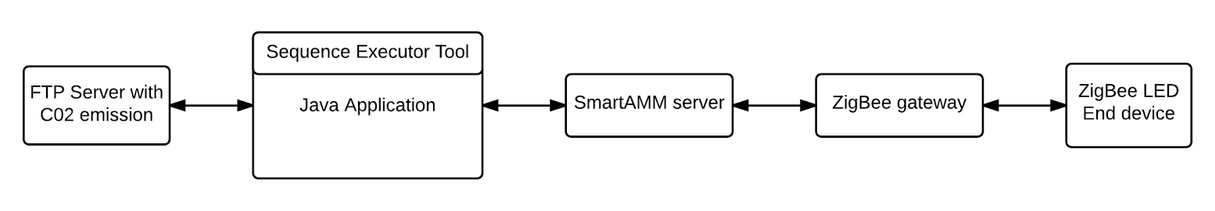
\includegraphics[width=\linewidth]{SystemDescription}
		\caption{System description}
		\label{fig:sysDesc}
		\end{figure}




	\subsection{Decision Making}



	\subsection{Sequence Executor Tool}
		The Sequence Executor Tool, which is provided by Develco Products, is a Java application able to communicate with ZigBee devices through a SmartAMM server.
		In order for this to work, two main files are needed: A setting file and a sequence file.
		


	\subsection{Application}



	\subsection{Communication Protocols}
		% Zigbee - Ivan Starter
		% Web protokoller - Ivan Starter
		% Det sidste



% section design_implementation_test_setup (end)
\end{document}